%% Figure 1 (pgfplots): Full-width 3-panel empirical overview & Block-2 silent-routing lag map with outward ticks and generous spacing.
\definecolor{stepc}{HTML}{0072B2}\definecolor{outc}{HTML}{D55E00}\definecolor{theoc}{HTML}{1E7E4E}
\definecolor{modelc}{HTML}{6A3D9A}\definecolor{mutedc}{HTML}{6E6E6E}
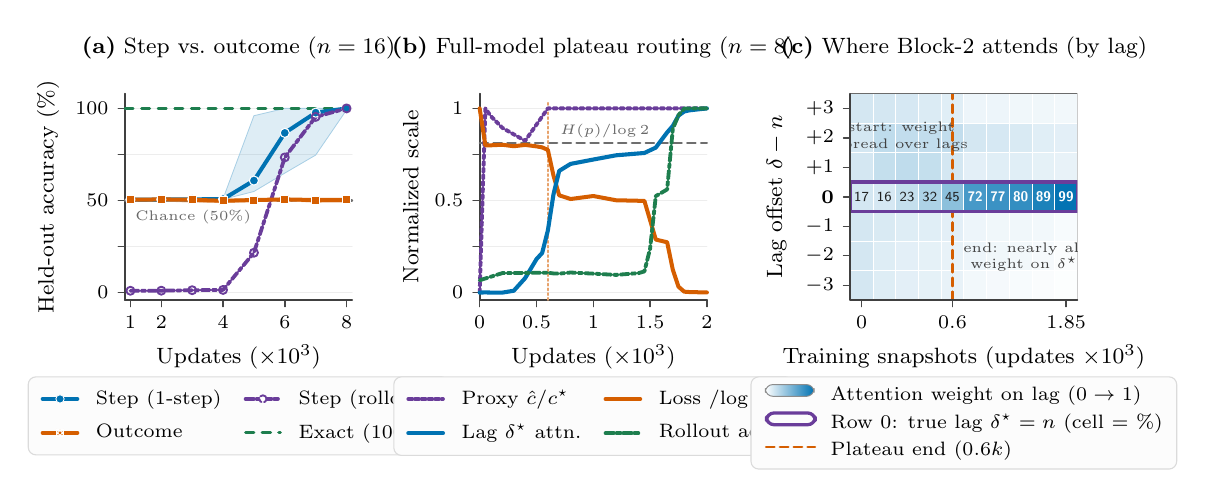
\begin{tikzpicture}[line cap=round, line join=round]
\pgfplotsset{
  every axis/.style={
    scale only axis,
    width=0.238\textwidth,
    height=2.62cm,
    axis line style={black!75, line width=0.64pt},
    tick align=outside,
    tickwidth=2.4pt,
    tick style={black!72, line width=0.52pt},
    tick label style={font=\scriptsize},
    label style={font=\footnotesize},
    ylabel style={yshift=-1pt},
    xlabel style={yshift=1pt},
    title style={font=\footnotesize, at={(0.5,1.04)}, anchor=south},
    axis x line*=bottom,
    axis y line*=left,
    legend style={
      at={(0.5,-0.37)},
      anchor=north,
      legend columns=2,
      font=\scriptsize,
      draw=black!14,
      fill=black!1.2,
      rounded corners=2.8pt,
      inner xsep=4.5pt,
      inner ysep=2.6pt,
      column sep=4pt,
      row sep=1.5pt,
      cells={anchor=west},
      /tikz/every even column/.append style={column sep=6pt}
    },
    legend image code/.code={
      \draw[#1] (0cm,0cm) -- (0.44cm,0cm);
    }
  },
  every axis plot/.append style={line width=1.42pt}
}

% (a) Step vs outcome (n=16, 10 paired seeds)
\begin{axis}[
  name=pa,
  title={\textbf{(a)} Step vs.\ outcome ($n=16$)},
  xlabel={Updates ($\times 10^3$)},
  ylabel={Held-out accuracy (\%)},
  xmin=0.82, xmax=8.18, ymin=-4, ymax=108,
  xtick={1,2,4,6,8},
  ytick={0,25,50,75,100},
  yticklabels={$0$,,$50$,,$100$},
  ymajorgrids, major grid style={black!7, line width=0.35pt},
  legend style={name=lega},
  clip=false
]
  \addplot[mutedc, densely dashed, line width=0.8pt, domain=0.82:8.18, samples=2, forget plot] {50};
  \node[anchor=north west, font=\tiny, text=mutedc!95!black, inner sep=1pt] at (axis cs:1.05,46.4) {Chance ($50\%$)};

  \addplot[draw=stepc!34, line width=0.3pt, fill=stepc, fill opacity=0.13, forget plot] coordinates {(1,50.28) (2,50.37) (3,50.41) (4,50.63) (5,54.89) (6,64.88) (7,74.67) (8,99.20) (8,100.00) (7,100.00) (6,100.00) (5,96.02) (4,50.95) (3,50.70) (2,50.68) (1,50.68)} -- cycle;
  \addplot[draw=outc!38, line width=0.3pt, fill=outc, fill opacity=0.14, forget plot] coordinates {(1,49.52) (2,49.73) (3,49.05) (4,48.92) (5,49.35) (6,49.92) (7,48.97) (8,49.15) (8,50.70) (7,50.70) (6,51.20) (5,51.08) (4,50.60) (3,50.70) (2,51.08) (1,51.08)} -- cycle;

  \addplot[theoc, dashed, line width=0.95pt, domain=0.82:8.18, samples=2, forget plot] {100};

  \addplot[
    stepc, solid, line width=1.45pt,
    mark=*, mark size=1.65pt,
    mark options={solid, fill=stepc, draw=white, line width=0.38pt},
    legend image code/.code={
      \draw[stepc, line width=1.45pt] (0cm,0cm) -- (0.44cm,0cm);
      \filldraw[fill=stepc, draw=white, line width=0.3pt] (0.22cm,0cm) circle[radius=1.5pt];
    }
  ] coordinates {(1,50.50) (2,50.53) (3,50.65) (4,50.73) (5,60.83) (6,86.70) (7,97.70) (8,100.00)};
  \addlegendentry{Step ($1$-step)}

  \addplot[
    modelc, densely dashdotted, line width=1.35pt,
    mark=o, mark size=1.45pt,
    mark options={solid, fill=white, draw=modelc, line width=0.68pt},
    legend image code/.code={
      \draw[modelc, densely dashdotted, line width=1.35pt] (0cm,0cm) -- (0.44cm,0cm);
      \filldraw[fill=white, draw=modelc, line width=0.68pt] (0.22cm,0cm) circle[radius=1.3pt];
    }
  ] coordinates {(1,1.00) (2,1.05) (3,1.30) (4,1.45) (5,21.65) (6,73.40) (7,95.40) (8,100.00)};
  \addlegendentry{Step (rollout)}

  \addplot[
    outc, solid, line width=1.45pt,
    mark=square*, mark size=1.45pt,
    mark options={solid, fill=outc, draw=white, line width=0.38pt},
    legend image code/.code={
      \draw[outc, line width=1.45pt] (0cm,0cm) -- (0.44cm,0cm);
      \filldraw[fill=outc, draw=white, line width=0.3pt] (0.175cm,-0.045cm) rectangle (0.265cm,0.045cm);
    }
  ] coordinates {(1,50.40) (2,50.60) (3,50.40) (4,49.85) (5,50.25) (6,50.60) (7,50.25) (8,50.40)};
  \addlegendentry{Outcome}

  \addlegendimage{theoc, dashed, line width=1.15pt}
  \addlegendentry{Exact ($100\%$)}
\end{axis}

% (b) Full 27-block Shortcut Denoising & Silent Routing trajectory (n=8, d=64)
\begin{axis}[
  name=pb,
  at={(pa.east)}, anchor=west, xshift=1.62cm,
  title={\textbf{(b)} Full-model plateau routing ($n=8$)},
  xlabel={Updates ($\times 10^3$)},
  ylabel={Normalized scale},
  xmin=0, xmax=2.0, ymin=-0.04, ymax=1.08,
  xtick={0,0.5,1,1.5,2},
  ytick={0,0.25,0.5,0.75,1},
  yticklabels={$0$,,$0.5$,,$1$},
  ymajorgrids, major grid style={black!7, line width=0.4pt},
  legend style={name=legb},
  clip=false
]
  \addplot[mutedc, densely dashed, line width=0.85pt, domain=0:2.0, samples=2, forget plot] {0.8113};
  \node[anchor=south, font=\tiny, text=mutedc!95!black, inner sep=1pt] at (axis cs:1.10,0.822) {$H(p)/\!\log 2$};
  \draw[outc!58, densely dotted, line width=0.72pt] (axis cs:0.60,-0.04) -- (axis cs:0.60,1.04);

  \addplot[modelc, densely dotted, line width=1.38pt] coordinates {(0.00,0.0000) (0.05,1.0000) (0.10,0.9568) (0.20,0.8943) (0.40,0.8241) (0.60,1.0000) (2.00,1.0000)};
  \addlegendentry{Proxy $\hat c/c^\star$}
  \addplot[outc, line width=1.45pt] coordinates {(0.00,1.0000) (0.05,0.7996) (0.10,0.7997) (0.20,0.8027) (0.30,0.7946) (0.40,0.8018) (0.50,0.7939) (0.55,0.7883) (0.60,0.7746) (0.65,0.6343) (0.70,0.5282) (0.80,0.5080) (1.00,0.5244) (1.20,0.5013) (1.45,0.4978) (1.55,0.2879) (1.65,0.2733) (1.70,0.1238) (1.75,0.0320) (1.80,0.0051) (1.85,0.0028) (2.00,0.0008)};
  \addlegendentry{Loss $\Lstep/\!\log 2$}
  \addplot[stepc, line width=1.48pt] coordinates {(0.00,0.0000) (0.05,0.0012) (0.10,0.0000) (0.20,0.0000) (0.30,0.0101) (0.40,0.0783) (0.50,0.1815) (0.55,0.2153) (0.60,0.3367) (0.65,0.5346) (0.70,0.6608) (0.80,0.6987) (1.00,0.7224) (1.20,0.7453) (1.45,0.7581) (1.55,0.7871) (1.65,0.8695) (1.70,0.9048) (1.75,0.9607) (1.80,0.9834) (1.85,0.9899) (2.00,1.0000)};
  \addlegendentry{Lag $\delta^\star$ attn.}
  \addplot[theoc, densely dashdotted, line width=1.38pt] coordinates {(0.00,0.0670) (0.20,0.1060) (0.40,0.1070) (0.60,0.1080) (0.65,0.1040) (0.70,0.1030) (0.80,0.1090) (1.00,0.1030) (1.20,0.0960) (1.40,0.1060) (1.45,0.1150) (1.50,0.2390) (1.55,0.5240) (1.65,0.5600) (1.70,0.8890) (1.75,0.9640) (1.80,0.9990) (1.85,1.0000) (2.00,1.0000)};
  \addlegendentry{Rollout acc.}
\end{axis}

% (c) Full 27-block Block-2 prefix-lag heatmap across training (outward ticks avoid '-17' illusion!)
\begin{axis}[
  name=pc,
  at={(pb.east)}, anchor=west, xshift=1.82cm,
  title={\textbf{(c)} Where Block-$2$ attends (by lag)},
  xlabel={Training snapshots (updates $\times 10^3$)},
  ylabel={Lag offset $\delta - n$},
  ylabel style={yshift=1pt},
  xmin=0, xmax=10, ymin=-3.5, ymax=3.5,
  xtick={0.5,4.5,9.5}, xticklabels={$0$,$0.6$,$1.85$},
  ytick={-3,-2,-1,0,1,2,3}, yticklabels={$-3$,$-2$,$-1$,$\mathbf{0}$,$+1$,$+2$,$+3$},
  axis line style={black!75, line width=0.55pt}, enlargelimits=false, axis on top
]
  \fill[stepc!17!white, draw=white, line width=0.3pt] (axis cs:0,-3.5) rectangle (axis cs:1,-2.5);
  \fill[stepc!17!white, draw=white, line width=0.3pt] (axis cs:0,-2.5) rectangle (axis cs:1,-1.5);
  \fill[stepc!17!white, draw=white, line width=0.3pt] (axis cs:0,-1.5) rectangle (axis cs:1,-0.5);
  \fill[stepc!17!white, draw=white, line width=0.3pt] (axis cs:0,-0.5) rectangle (axis cs:1,0.5);
  \fill[stepc!17!white, draw=white, line width=0.3pt] (axis cs:0,0.5) rectangle (axis cs:1,1.5);
  \fill[stepc!17!white, draw=white, line width=0.3pt] (axis cs:0,1.5) rectangle (axis cs:1,2.5);
  \fill[stepc!17!white, draw=white, line width=0.3pt] (axis cs:0,2.5) rectangle (axis cs:1,3.5);
  \fill[stepc!13!white, draw=white, line width=0.3pt] (axis cs:1,-3.5) rectangle (axis cs:2,-2.5);
  \fill[stepc!13!white, draw=white, line width=0.3pt] (axis cs:1,-2.5) rectangle (axis cs:2,-1.5);
  \fill[stepc!15!white, draw=white, line width=0.3pt] (axis cs:1,-1.5) rectangle (axis cs:2,-0.5);
  \fill[stepc!16!white, draw=white, line width=0.3pt] (axis cs:1,-0.5) rectangle (axis cs:2,0.5);
  \fill[stepc!23!white, draw=white, line width=0.3pt] (axis cs:1,0.5) rectangle (axis cs:2,1.5);
  \fill[stepc!25!white, draw=white, line width=0.3pt] (axis cs:1,1.5) rectangle (axis cs:2,2.5);
  \fill[stepc!17!white, draw=white, line width=0.3pt] (axis cs:1,2.5) rectangle (axis cs:2,3.5);
  \fill[stepc!11!white, draw=white, line width=0.3pt] (axis cs:2,-3.5) rectangle (axis cs:3,-2.5);
  \fill[stepc!11!white, draw=white, line width=0.3pt] (axis cs:2,-2.5) rectangle (axis cs:3,-1.5);
  \fill[stepc!13!white, draw=white, line width=0.3pt] (axis cs:2,-1.5) rectangle (axis cs:3,-0.5);
  \fill[stepc!23!white, draw=white, line width=0.3pt] (axis cs:2,-0.5) rectangle (axis cs:3,0.5);
  \fill[stepc!25!white, draw=white, line width=0.3pt] (axis cs:2,0.5) rectangle (axis cs:3,1.5);
  \fill[stepc!24!white, draw=white, line width=0.3pt] (axis cs:2,1.5) rectangle (axis cs:3,2.5);
  \fill[stepc!16!white, draw=white, line width=0.3pt] (axis cs:2,2.5) rectangle (axis cs:3,3.5);
  \fill[stepc!10!white, draw=white, line width=0.3pt] (axis cs:3,-3.5) rectangle (axis cs:4,-2.5);
  \fill[stepc!10!white, draw=white, line width=0.3pt] (axis cs:3,-2.5) rectangle (axis cs:4,-1.5);
  \fill[stepc!12!white, draw=white, line width=0.3pt] (axis cs:3,-1.5) rectangle (axis cs:4,-0.5);
  \fill[stepc!32!white, draw=white, line width=0.3pt] (axis cs:3,-0.5) rectangle (axis cs:4,0.5);
  \fill[stepc!23!white, draw=white, line width=0.3pt] (axis cs:3,0.5) rectangle (axis cs:4,1.5);
  \fill[stepc!24!white, draw=white, line width=0.3pt] (axis cs:3,1.5) rectangle (axis cs:4,2.5);
  \fill[stepc!14!white, draw=white, line width=0.3pt] (axis cs:3,2.5) rectangle (axis cs:4,3.5);
  \fill[stepc!9!white, draw=white, line width=0.3pt] (axis cs:4,-3.5) rectangle (axis cs:5,-2.5);
  \fill[stepc!9!white, draw=white, line width=0.3pt] (axis cs:4,-2.5) rectangle (axis cs:5,-1.5);
  \fill[stepc!11!white, draw=white, line width=0.3pt] (axis cs:4,-1.5) rectangle (axis cs:5,-0.5);
  \fill[stepc!45!white, draw=white, line width=0.3pt] (axis cs:4,-0.5) rectangle (axis cs:5,0.5);
  \fill[stepc!17!white, draw=white, line width=0.3pt] (axis cs:4,0.5) rectangle (axis cs:5,1.5);
  \fill[stepc!24!white, draw=white, line width=0.3pt] (axis cs:4,1.5) rectangle (axis cs:5,2.5);
  \fill[stepc!12!white, draw=white, line width=0.3pt] (axis cs:4,2.5) rectangle (axis cs:5,3.5);
  \fill[stepc!5!white, draw=white, line width=0.3pt] (axis cs:5,-3.5) rectangle (axis cs:6,-2.5);
  \fill[stepc!7!white, draw=white, line width=0.3pt] (axis cs:5,-2.5) rectangle (axis cs:6,-1.5);
  \fill[stepc!7!white, draw=white, line width=0.3pt] (axis cs:5,-1.5) rectangle (axis cs:6,-0.5);
  \fill[stepc!72!white, draw=white, line width=0.3pt] (axis cs:5,-0.5) rectangle (axis cs:6,0.5);
  \fill[stepc!11!white, draw=white, line width=0.3pt] (axis cs:5,0.5) rectangle (axis cs:6,1.5);
  \fill[stepc!17!white, draw=white, line width=0.3pt] (axis cs:5,1.5) rectangle (axis cs:6,2.5);
  \fill[stepc!7!white, draw=white, line width=0.3pt] (axis cs:5,2.5) rectangle (axis cs:6,3.5);
  \fill[stepc!4!white, draw=white, line width=0.3pt] (axis cs:6,-3.5) rectangle (axis cs:7,-2.5);
  \fill[stepc!6!white, draw=white, line width=0.3pt] (axis cs:6,-2.5) rectangle (axis cs:7,-1.5);
  \fill[stepc!6!white, draw=white, line width=0.3pt] (axis cs:6,-1.5) rectangle (axis cs:7,-0.5);
  \fill[stepc!77!white, draw=white, line width=0.3pt] (axis cs:6,-0.5) rectangle (axis cs:7,0.5);
  \fill[stepc!12!white, draw=white, line width=0.3pt] (axis cs:6,0.5) rectangle (axis cs:7,1.5);
  \fill[stepc!16!white, draw=white, line width=0.3pt] (axis cs:6,1.5) rectangle (axis cs:7,2.5);
  \fill[stepc!7!white, draw=white, line width=0.3pt] (axis cs:6,2.5) rectangle (axis cs:7,3.5);
  \fill[stepc!3!white, draw=white, line width=0.3pt] (axis cs:7,-3.5) rectangle (axis cs:8,-2.5);
  \fill[stepc!5!white, draw=white, line width=0.3pt] (axis cs:7,-2.5) rectangle (axis cs:8,-1.5);
  \fill[stepc!6!white, draw=white, line width=0.3pt] (axis cs:7,-1.5) rectangle (axis cs:8,-0.5);
  \fill[stepc!80!white, draw=white, line width=0.3pt] (axis cs:7,-0.5) rectangle (axis cs:8,0.5);
  \fill[stepc!12!white, draw=white, line width=0.3pt] (axis cs:7,0.5) rectangle (axis cs:8,1.5);
  \fill[stepc!15!white, draw=white, line width=0.3pt] (axis cs:7,1.5) rectangle (axis cs:8,2.5);
  \fill[stepc!6!white, draw=white, line width=0.3pt] (axis cs:7,2.5) rectangle (axis cs:8,3.5);
  \fill[stepc!2!white, draw=white, line width=0.3pt] (axis cs:8,-3.5) rectangle (axis cs:9,-2.5);
  \fill[stepc!4!white, draw=white, line width=0.3pt] (axis cs:8,-2.5) rectangle (axis cs:9,-1.5);
  \fill[stepc!5!white, draw=white, line width=0.3pt] (axis cs:8,-1.5) rectangle (axis cs:9,-0.5);
  \fill[stepc!89!white, draw=white, line width=0.3pt] (axis cs:8,-0.5) rectangle (axis cs:9,0.5);
  \fill[stepc!10!white, draw=white, line width=0.3pt] (axis cs:8,0.5) rectangle (axis cs:9,1.5);
  \fill[stepc!12!white, draw=white, line width=0.3pt] (axis cs:8,1.5) rectangle (axis cs:9,2.5);
  \fill[stepc!6!white, draw=white, line width=0.3pt] (axis cs:8,2.5) rectangle (axis cs:9,3.5);
  \fill[stepc!1!white, draw=white, line width=0.3pt] (axis cs:9,-3.5) rectangle (axis cs:10,-2.5);
  \fill[stepc!2!white, draw=white, line width=0.3pt] (axis cs:9,-2.5) rectangle (axis cs:10,-1.5);
  \fill[stepc!3!white, draw=white, line width=0.3pt] (axis cs:9,-1.5) rectangle (axis cs:10,-0.5);
  \fill[stepc!99!white, draw=white, line width=0.3pt] (axis cs:9,-0.5) rectangle (axis cs:10,0.5);
  \fill[stepc!9!white, draw=white, line width=0.3pt] (axis cs:9,0.5) rectangle (axis cs:10,1.5);
  \fill[stepc!11!white, draw=white, line width=0.3pt] (axis cs:9,1.5) rectangle (axis cs:10,2.5);
  \fill[stepc!5!white, draw=white, line width=0.3pt] (axis cs:9,2.5) rectangle (axis cs:10,3.5);
  \draw[outc, densely dashed, line width=0.95pt] (axis cs:4.5,-3.5) -- (axis cs:4.5,-0.5);
  \draw[outc, densely dashed, line width=0.95pt] (axis cs:4.5,0.5) -- (axis cs:4.5,3.5);
  \draw[black!58, line width=0.48pt] (axis cs:0,-3.5) rectangle (axis cs:10,3.5);
  % Target-lag row: bold royal-purple outline plus clean percentage values
  \draw[modelc, line width=1.18pt] (axis cs:0,-0.5) rectangle (axis cs:10,0.5);
  \node[font=\tiny\sffamily, text=black!88] at (axis cs:0.5,0) {17};
  \node[font=\tiny\sffamily, text=black!88] at (axis cs:1.5,0) {16};
  \node[font=\tiny\sffamily, text=black!88] at (axis cs:2.5,0) {23};
  \node[font=\tiny\sffamily, text=black!88] at (axis cs:3.5,0) {32};
  \node[font=\tiny\sffamily, text=black!88] at (axis cs:4.5,0) {45};
  \node[font=\tiny\sffamily\bfseries, text=white] at (axis cs:5.5,0) {72};
  \node[font=\tiny\sffamily\bfseries, text=white] at (axis cs:6.5,0) {77};
  \node[font=\tiny\sffamily\bfseries, text=white] at (axis cs:7.5,0) {80};
  \node[font=\tiny\sffamily\bfseries, text=white] at (axis cs:8.5,0) {89};
  \node[font=\tiny\sffamily\bfseries, text=white] at (axis cs:9.5,0) {99};
  % Plain-language annotations
  \node[font=\tiny, align=center, text=black!75] at (axis cs:2.25,2.05) {start: weight\\spread over lags};
  \node[font=\tiny, align=center, text=black!75] at (axis cs:7.65,-2.05) {end: nearly all\\weight on $\delta^\star$};
\end{axis}

% External legend box under (c), top-aligned with (a) and (b) legend boxes
\node[
  at={(pc.south |- legb.north)},
  anchor=north,
  draw=black!14,
  fill=black!1.2,
  rounded corners=2.8pt,
  inner xsep=5pt,
  inner ysep=2.6pt,
  font=\scriptsize
] {
  \begin{tabular}{@{}l@{\hspace{5pt}}l@{}}
    \tikz[baseline=-0.5ex]{
      \shade[left color=white, right color=stepc] (0,0) rectangle (0.62cm,0.15cm);
      \draw[black!45, line width=0.35pt] (0,0) rectangle (0.62cm,0.15cm);
    } & Attention weight on lag ($0 \to 1$) \\[1.5pt]
    \tikz[baseline=-0.5ex]{
      \draw[modelc, line width=1.18pt] (0,0) rectangle (0.62cm,0.15cm);
    } & Row $0$: true lag $\delta^\star = n$ (cell = \%) \\[1.5pt]
    \tikz[baseline=-0.5ex]{
      \draw[outc, densely dashed, line width=0.95pt] (0,0.05cm) -- (0.62cm,0.05cm);
    } & Plateau end ($0.6\text{k}$)
  \end{tabular}
};
\end{tikzpicture}
